\documentclass{article}

\usepackage{../../common/labconfig}
\usepackage{../../common/labstyle}

\lhead{LIS3DH \& SPI Lab}

\begin{document}

\section{Introduction}

In this lab, you will use the ATMega328P's SPI controller to interface with an
LIS3DH accelerometer. You will also implement software-driven PWM to control
LEDs, using their intensity to indicate the force reading along each axis of
the accelerometer.

\begin{figure}[H]

	\centering

	\begin{tabular}{r|l}

		Part & Due Date \\ \hline\hline
		Part A & Feb. 28\\ \hline
		Part B & Mar. 6\\ \hline
		Part C & Mar. 13\\ \hline
		Reflection & Mar. 13\\ \hline

	\end{tabular}

	\caption{Table of due dates for each part.}

\end{figure}

\tableofcontents

\section{Parts List}

\begin{multicols}{2}

\begin{itemize}

\item one Adafruit Metro 328\footnote{Or compatible development board with an ATMega328P.}

\item six LEDs

\item several male-male jumper wires

\item several male-female jumper wiers

\item one USB cable

\item one breadboard

\item one LIS3DH breakout board

\item six 330$\Omega$ resistor (orange, orange, brown, gold)\footnote{Larger
	resistor may be substituted if needed.}

\item AVRIce Programmer and cables

\end{itemize}

\end{multicols}

\begin{figure}[H]
	\centering

	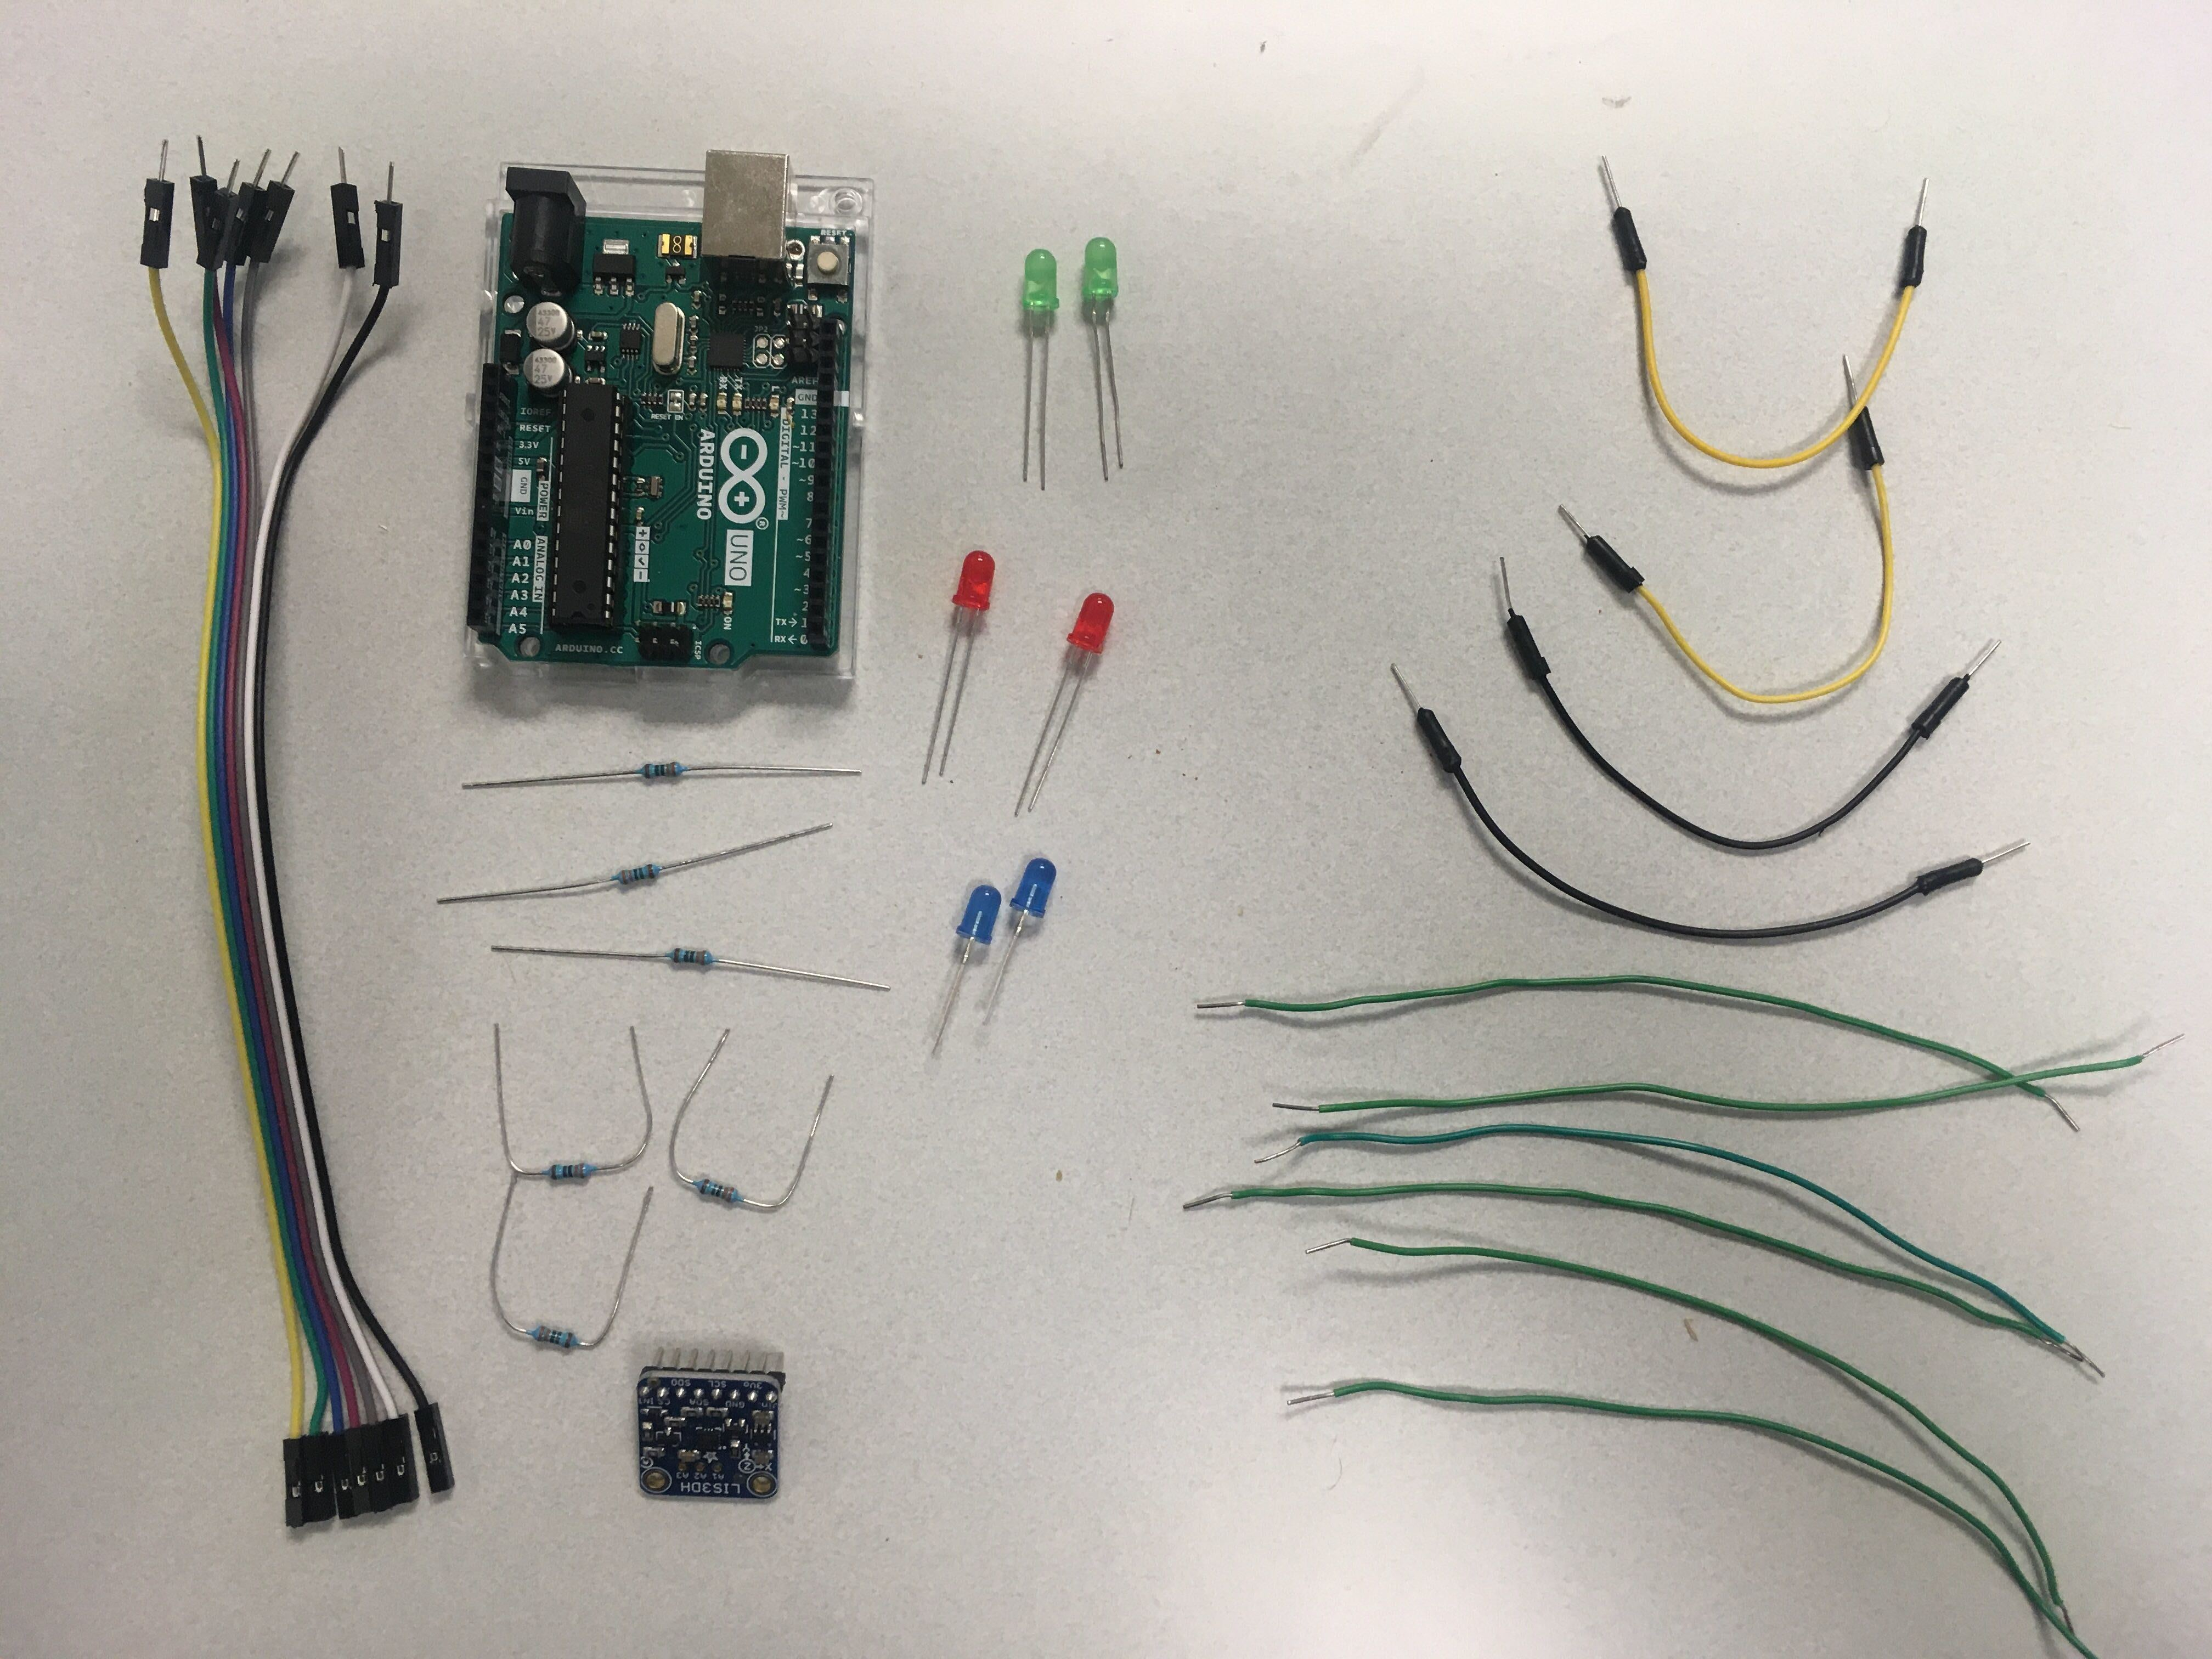
\includegraphics[max width = 0.7\textwidth]{parts.jpg}

	\caption{Photo showing parts for this project. Programmer and cables
	are not pictured, but are also needed. }

\end{figure}


\section{Part A: LIS3DH Data Readout}

\subsection{Wiring}


\begin{figure}[H]
	\centering

	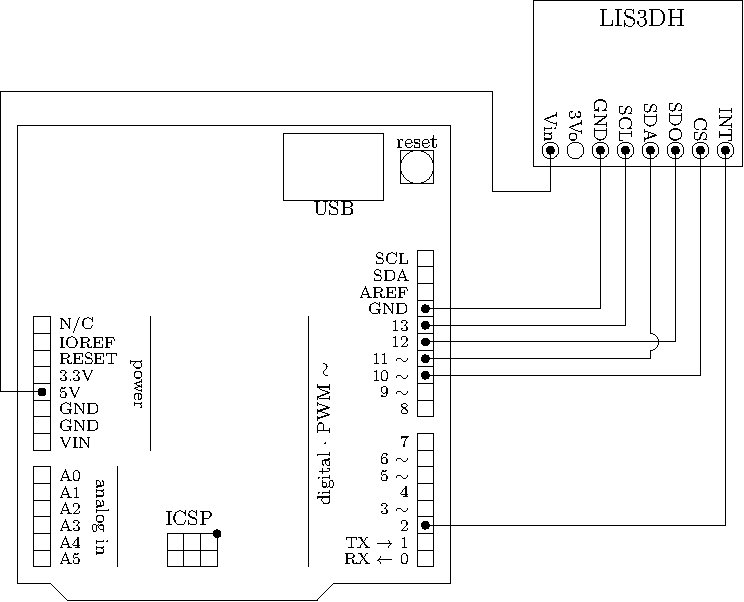
\includegraphics[max width = 0.7\textwidth]{part_a_wiring.pdf}

	\caption{Wiring diagram for part A.}

\end{figure}

\begin{figure}[H]

	\centering

	\begin{tabular}{|c|c|c|}

		\hline
		LIS3DH Pin & Metro 328 Pin & ATMega328P Pin \\
		\hline\hline

		Vin & 5V & 5V \\ \hline
		3Vo & N/C & N/C \\ \hline
		GND & GND & GND \\ \hline
		SCL & 13 & PB5/SCK/PCINT5 \\ \hline
		SDA & $\sim$ 11 & PB3/MOSI/OC2A/PCINT3 \\ \hline
		SDO & 12 & PB4/MISO/PCINT4 \\ \hline
		CS & $\sim$ 10 & PB2/SS/OC1B/PINT2 \\ \hline
		INT & 2 & PD2/INT0/PCINT18 \\ \hline

	\end{tabular}

	\caption{Table showing correct connections for Part A.}

\end{figure}


You should also connect the USB cable from your Arduino to your workstation.
This is how you will connect to the UART console.

Finally, connect the AVRIce programmer to your workstation, and the programming
cable to the Arduino. Remember that the tab on the programming cable should be
facing the interior of the Arduino board.

\begin{figure}[H]
	\centering

	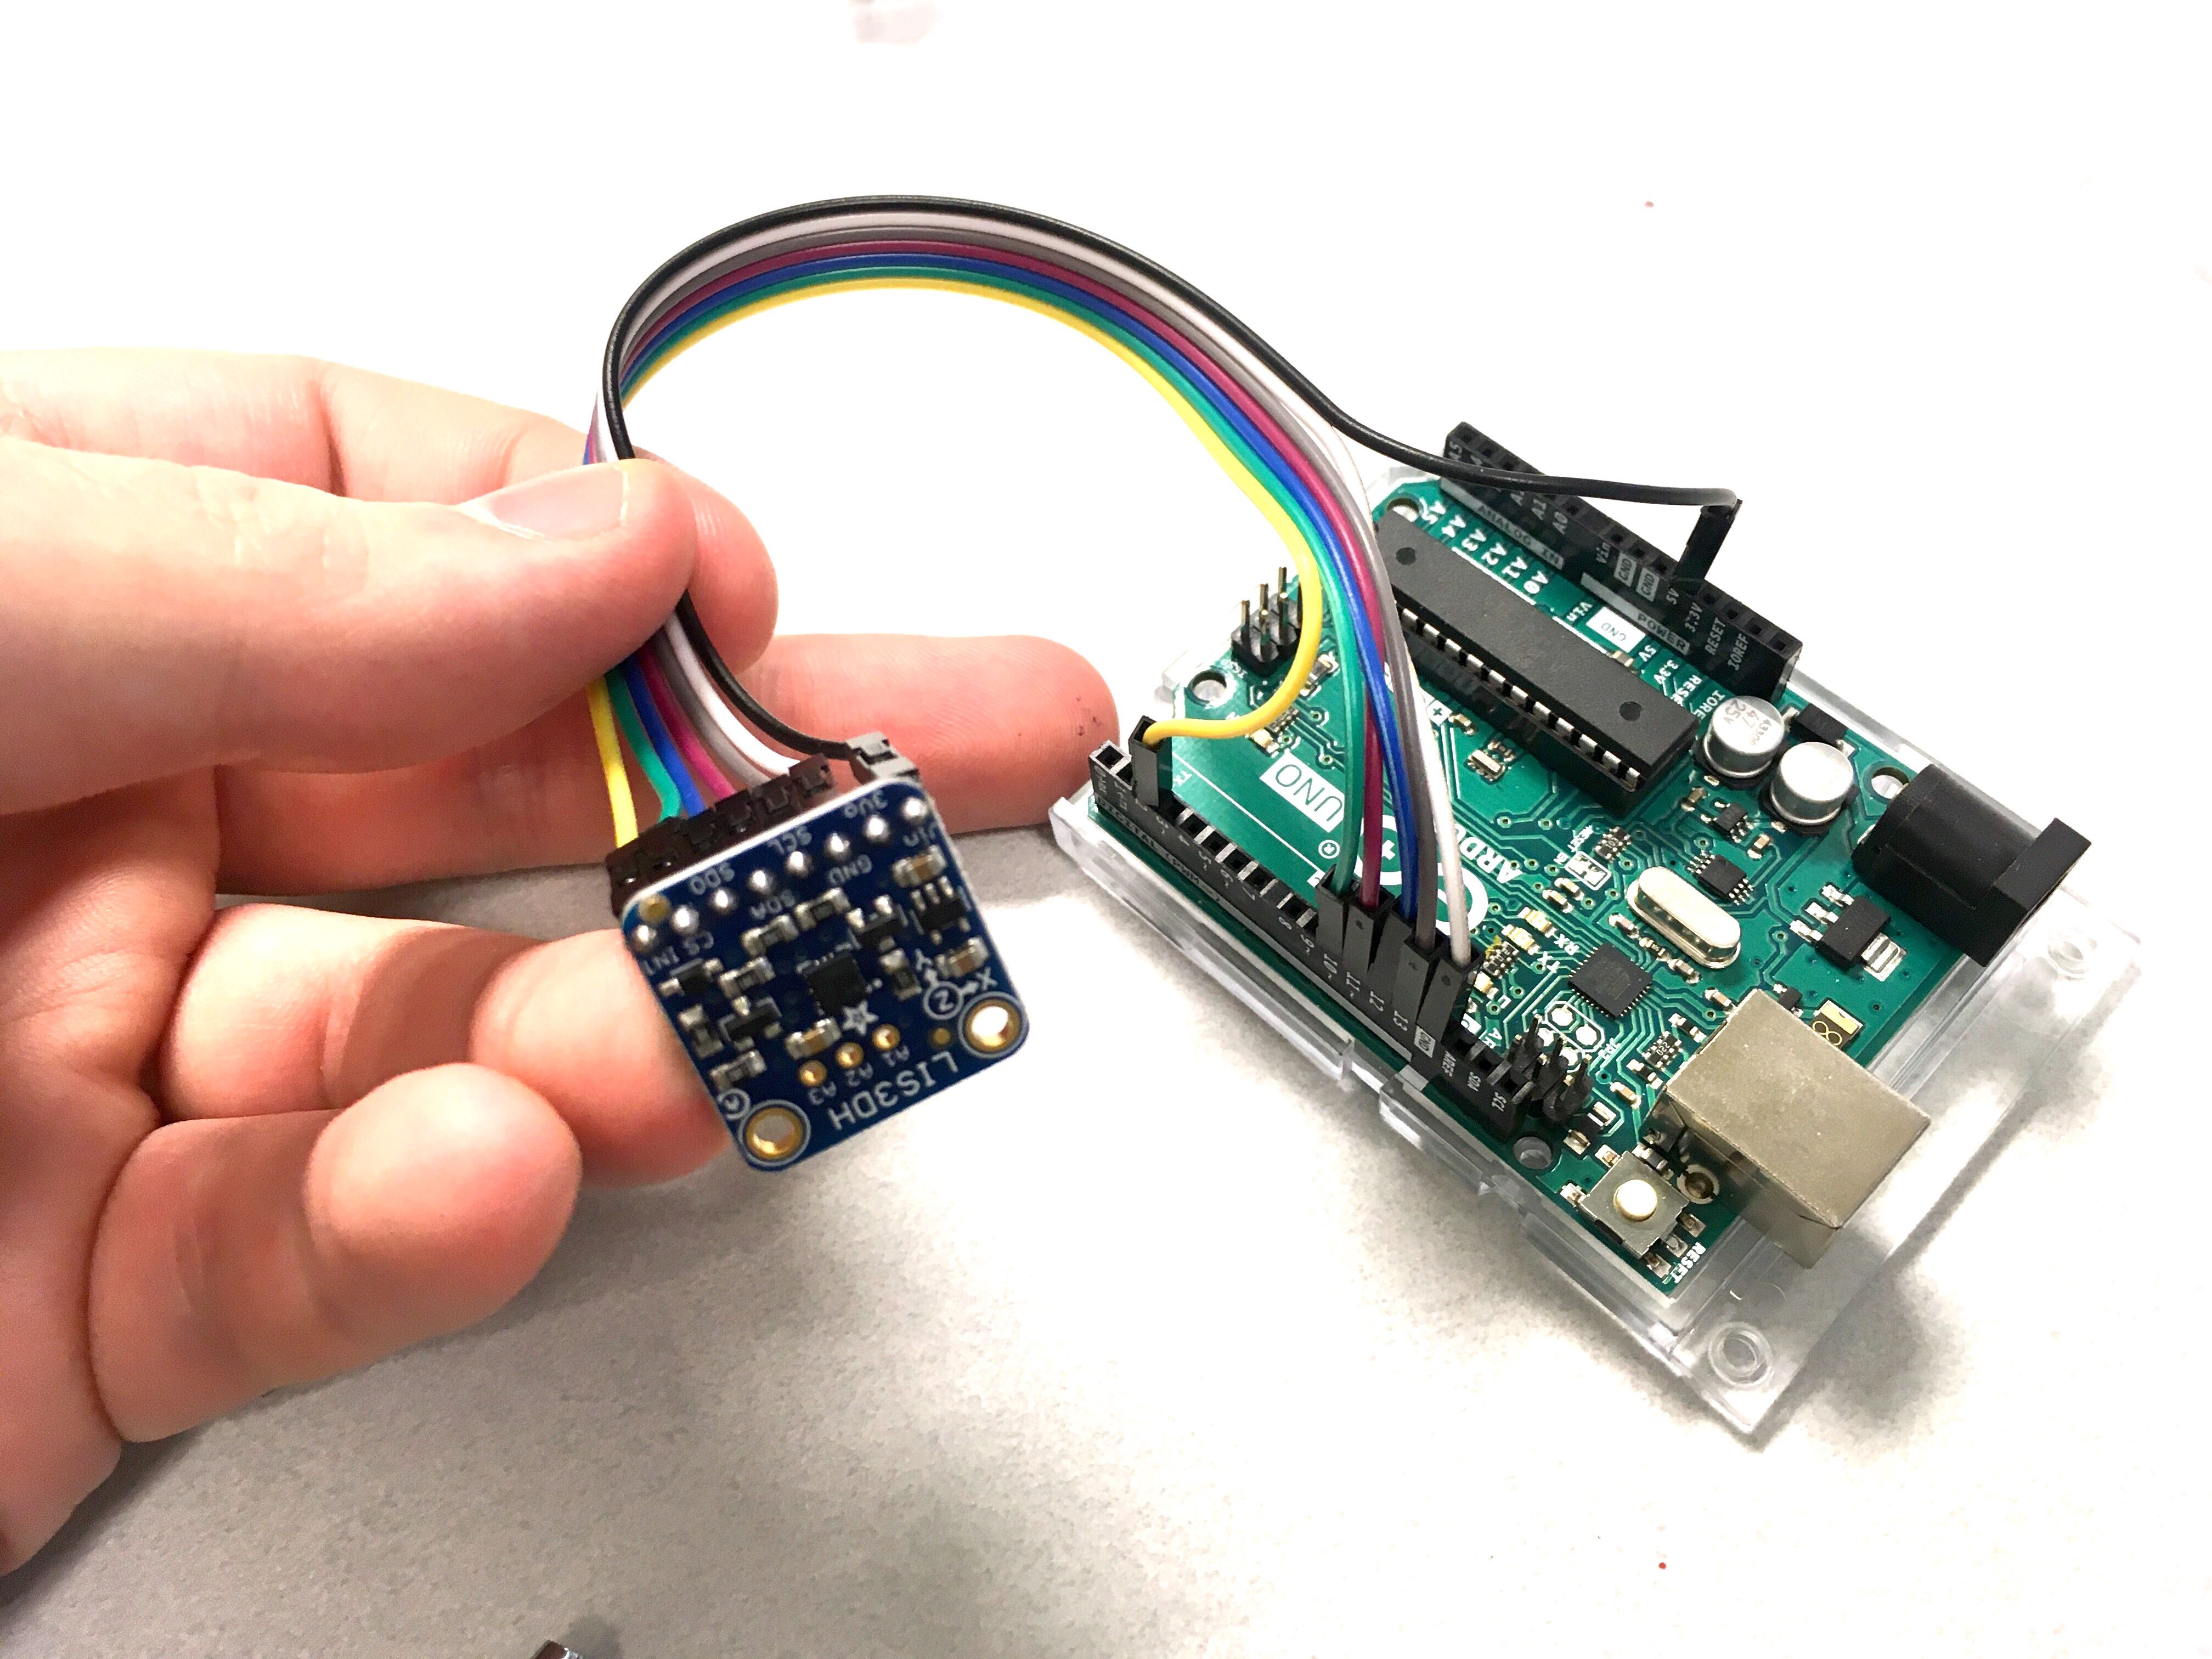
\includegraphics[max width = 0.7\textwidth]{wiring_part_a.jpg}

	\caption{Photograph showing correctly wired project for part A
	(programmer and cables not pictured).}

\end{figure}

If you want to validate your wiring, you can use \texttt{make wiringtest} which
will flash a test program to the board. Below are shown the expected outputs
if the LIS3DH is wired correctly, or if it is wired incorrectly.

\begin{lstlisting}[caption={\texttt{make wiringtest} output with \textbf{correct} wiring.}]
UART initialized (57600 8N1)


SPI initialized
initialization complete.


WHO_AM_I register read successfully!
Initial register values:
CTRL_REG0: 0x07
CTRL_REG1: 0x00
CTRL_REG2: 0x00
CTRL_REG3: 0x00
CTRL_REG4: 0x00
CTRL_REG5: 0x00
\end{lstlisting}


\begin{lstlisting}[caption={\texttt{make wiringtest} output with \textbf{incorrect} wiring.}]
UART initialized (57600 8N1)


SPI initialized
initialization complete.


WHO_AM_I register read failed!

Expected 0x33, got 0x0
Initial register values:
CTRL_REG0: 0x00
CTRL_REG1: 0x00
CTRL_REG2: 0x00
CTRL_REG3: 0x00
CTRL_REG4: 0x00
CTRL_REG5: 0x00
\end{lstlisting}

\subsection{Requirements}

\begin{itemize}

	\item (A.1) Your program should interface with the LIS3DH using SPI,
		and display the raw readings on each axis once per second
		over UART.

\end{itemize}

\subsection{Grading}

You do not need to submit any code for this portion. During lab, office hours,
or by appointment, demonstrate your project to your TA or instructor.

\subsection{Commentary}

To avoid wasting many cycles polling, you will want to configure the LIS3DH to provide external interrupts to the ATMega. Once things are configured correctly, the code should be fairly simple.

You will need to set \texttt{CTRL\_REG5} to disable the FIFO, and latch interrupts. You will then want to set the \texttt{FIFO\_CTRL\_REG} to run in Bypass mode. Then you will want to set \texttt{CTRL\_REG3} to enable the \texttt{DRDY1} interrupt. Lastly, set \texttt{CTRL\_REG6} to allow the INT1 interrupt on the LIS3DH to be active low.

If you correctly wrangled all of those settings, you can then configure the ATMega to detect external active low interrupts, and in the ISR, you will first read the \texttt{STATUS\_REG} register (to acknowledge/reset the interrupt), and then you can read the 6 output registers as normal.


\section{Part B: LED Indicators}

\subsection{Wiring}

For part B, you will connect six LEDs, each of which will be used to signify
the intensity of the accelerated reading along the marked axis. Note that you
will not be using the LIS3DH in this part, so you may optionally disconnect it.

\begin{figure}[H]
	\centering

	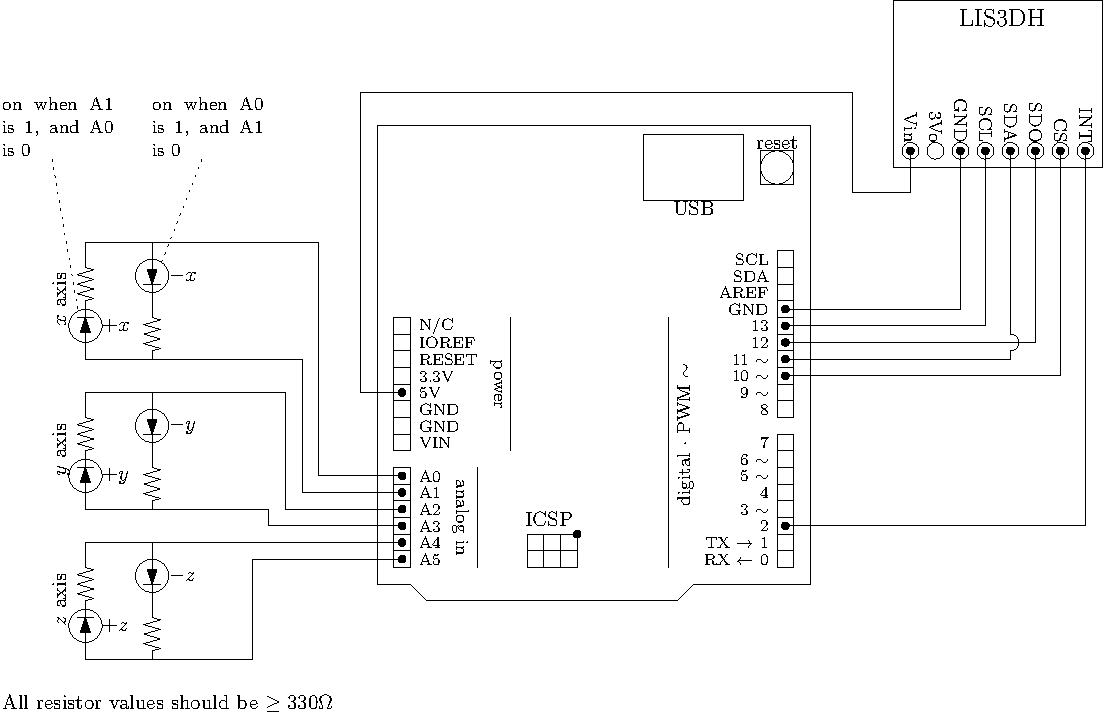
\includegraphics[max width = 0.9\textwidth]{part_b_wiring.pdf}

	\caption{Wiring diagram for part B.}

\end{figure}

You will need to connect six LEDs. Each pair of pins in A0 $\dots$ A5, is used
to drive one pair of LEDs - since the GPIO pins can be configured as positive
or negative (pull up or pull down), thus allowing either LED in a pair to be
activated at any given time.

You can test if your wiring is correct using the command \texttt{make
blinkenlights}. This will allow you to toggle each LED on or off individually
using the UART console (all LEDs will be off until you turn one on).

\begin{figure}[H]
	\centering

	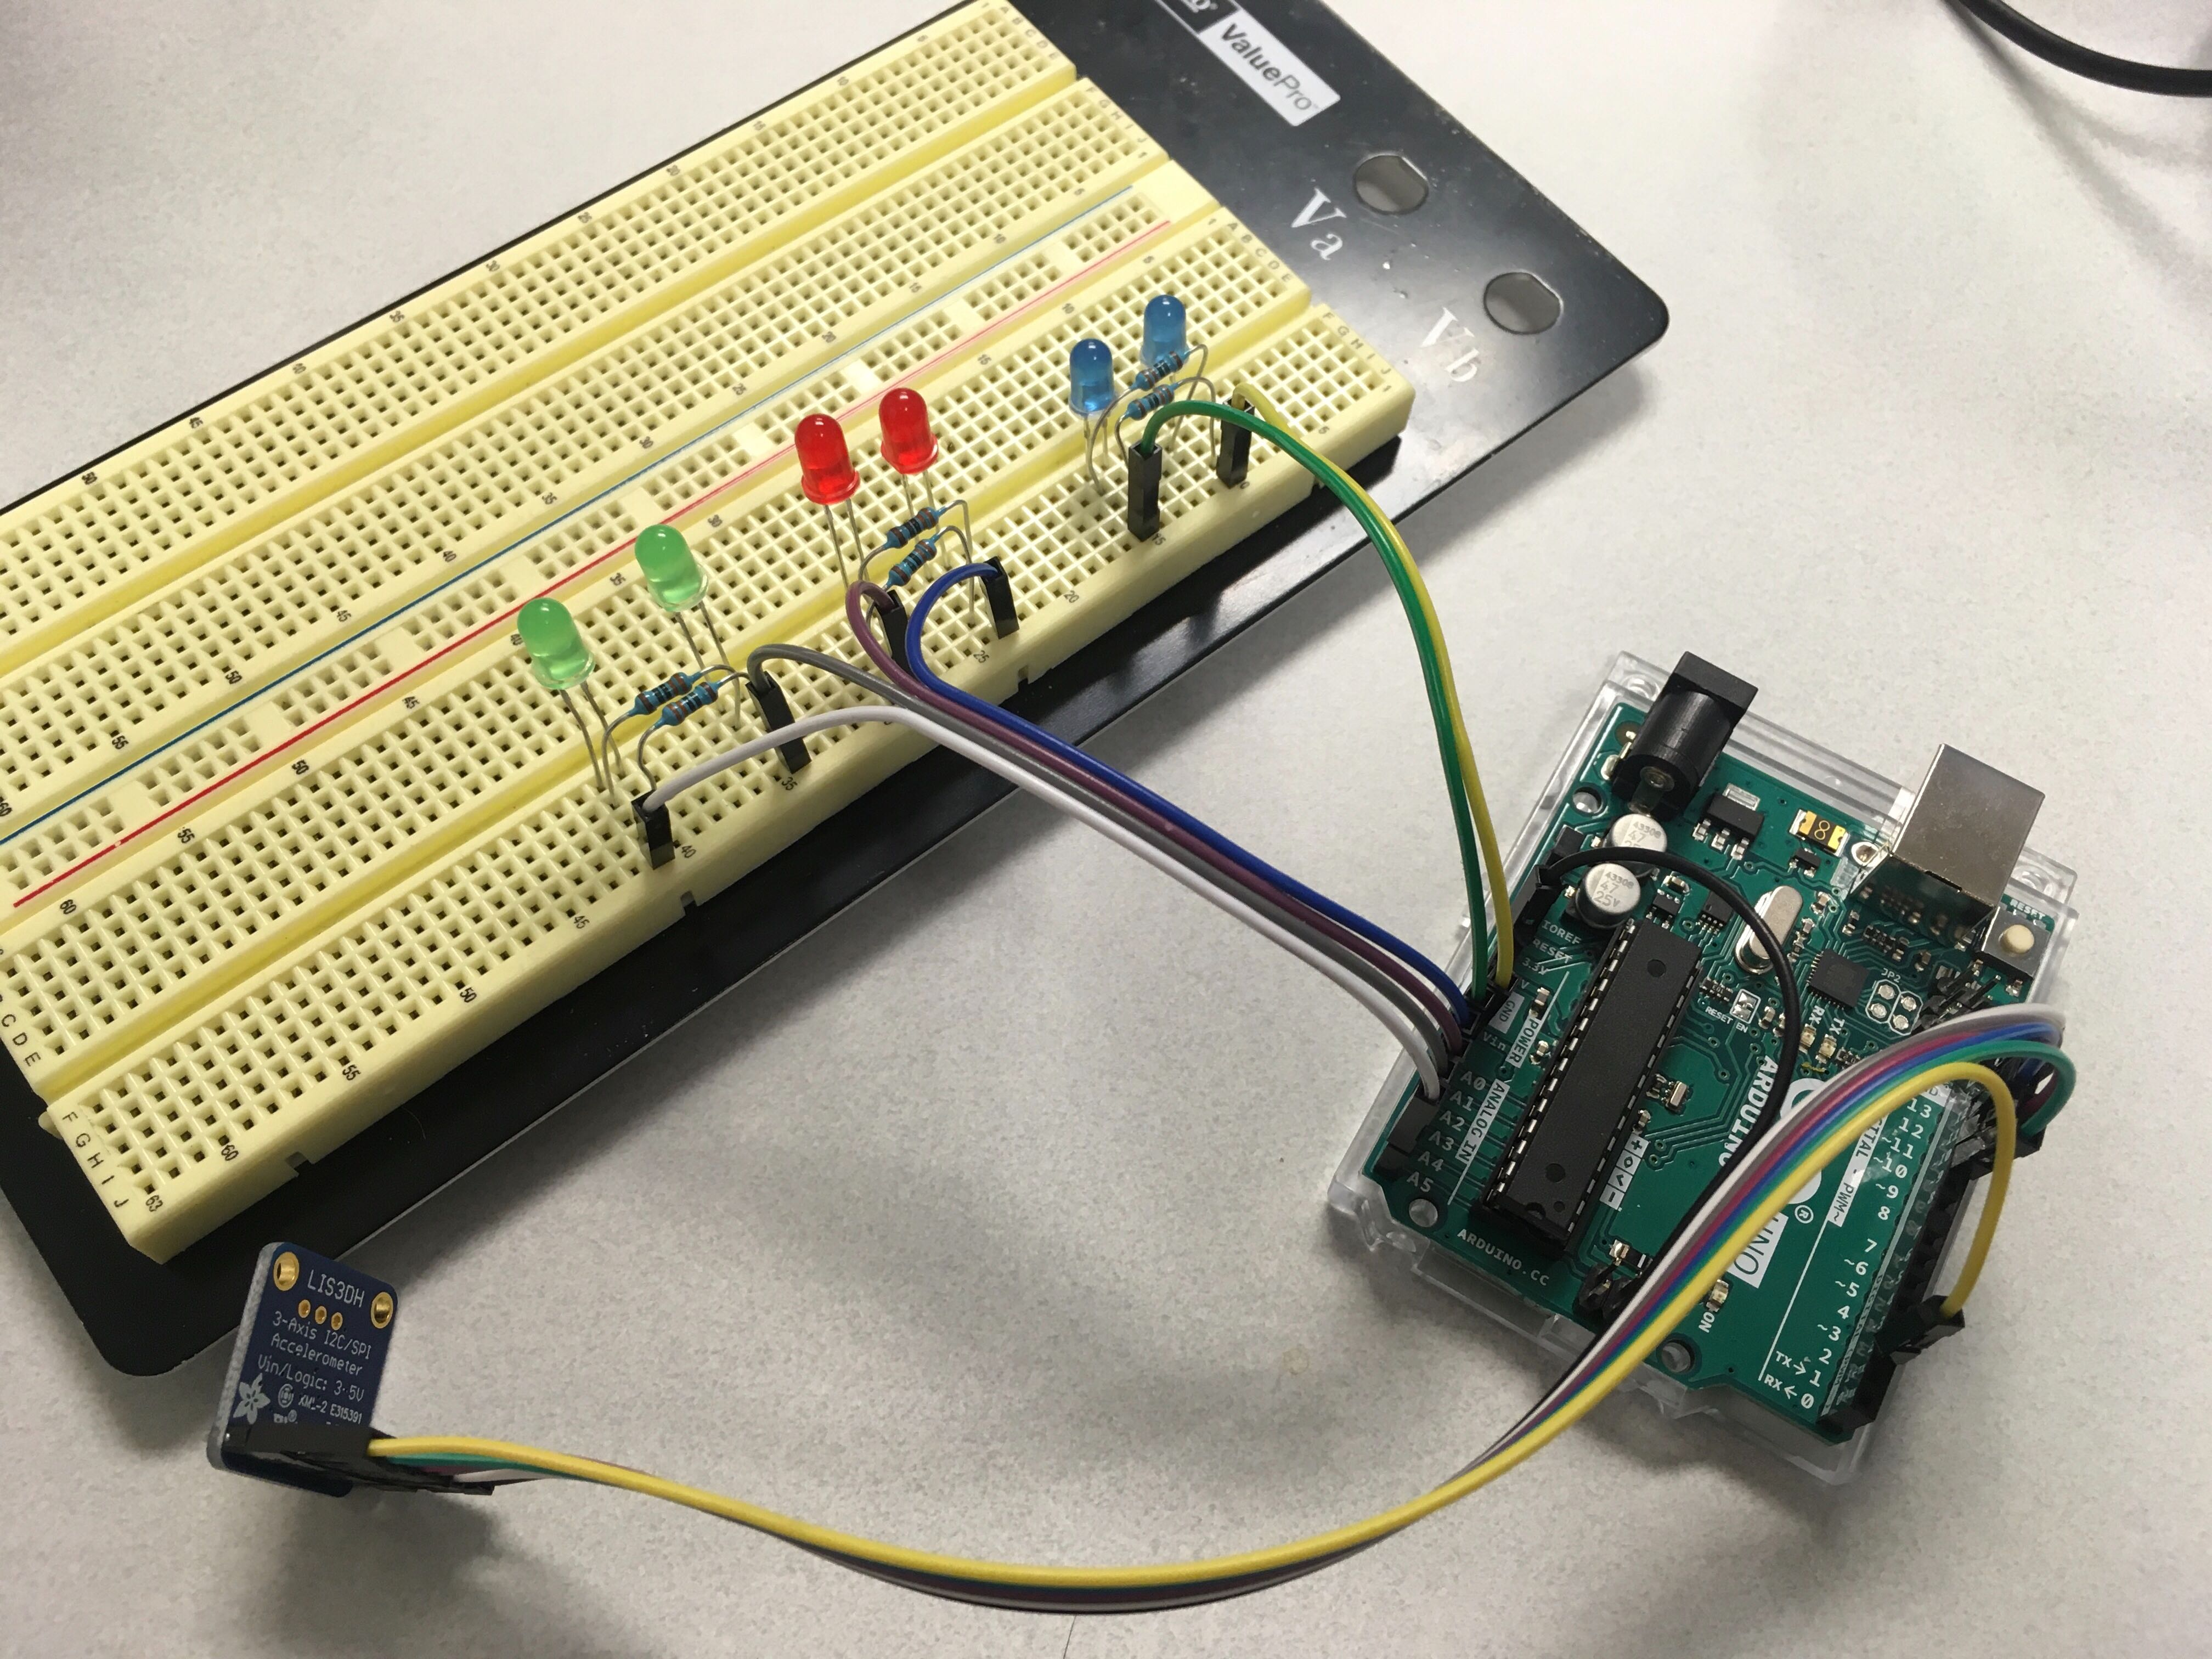
\includegraphics[max width = 0.7\textwidth]{wiring_part_b.jpg}

	\caption{Photograph showing correctly wired project for part B
	(programmer and cables not pictured).}

\end{figure}

\subsection{Requirements}

\begin{itemize}

	\item (B.1) Your program should expose an interactive command-line over
		UART. You should be able to enter three signed floating point
		values in the range $0.0\dots1.0$, in the format \texttt{"\%f
		\%f \%f"}. These values should represent "fake" sensor data for
		the $x$, $y$, and $z$ axes respectively. You may implement
		other commands for your own debugging purposes as desired.

	\item (B.2) LEDs should take on a level of brightness proportional to
		the specified axis values. For example, if the user inputs
		\texttt{1.0 0.3 -0.7}, then the $+x$ LED should run at full
		brightness, the $+y$ LED should run at 30\% brightness, and
		the $-z$ LED should run at 70\% brightness. The $-x$, $-y$, and
		$+z$ LEDs should all be completely off.


\end{itemize}

\subsection{Grading}

You do not need to submit any code for this portion. During lab, office hours,
or by appointment, demonstrate your project to your TA or instructor.

\subsection{Commentary}

This part segues into part C, in that you will simply be modifying your code to
compute the duty cycles for each LED from data read from the LIS3DH, rather
than the console.

As the ATMega328P has only two hardware PWM controllers, you will need to
implement software PWM. To avoid floating point math, it is suggested that you
should internally represent the PWM duty cycle as a \texttt{uint8\_t}.

\section{Part C: Combining the LIS3DH and LEDs}

\subsection{Wiring}

The wiring for this part is unmodified from part B, except that LIS3DH sensor
should be connected to the board if you disconnected it for part B.

\subsection{Requirements}

\begin{itemize}

	\item (C.1) When the LIS3DH sensor is rotated, the LED brightness
		should change to show the intensity of the sensor reading. For
		example, when the LIS3DH is accelerated along it's $+x$ axis,
		the $+x$ LED should be illuminated brightly.

	\item (C.2) The LEDs should not flicker, and should have no perceptible
		delay before updating. The interrupt rate of the LIS3DH should
		be set to at least 25Hz.

\end{itemize}

\subsection{Commentary}

Although it was possible in part A to interface with the LIS3DH using either a
polling or interrupt driven approach, part C will be much easier to complete
successfully with an interrupt-driven method.

\section{Reflection}

\textbf{You should submit your answers by editing \texttt{reflection.txt} to
include them before you run \texttt{make pack}}.  There is no specific
requirement for word or page count, but roughly 1-3 paragraphs are expected in
response to each question. Note that your reflection will be graded with your
submission to part D.


\subsection{Question 1}

For what reason might the \texttt{WHO\_AM\_I} register be included in the design
of the LIS3DH? What negative impacts might there be if it were omitted?

\subsection{Question 2}

What value should be written to the LIS3DH's \texttt{CTRL\_REG1} in order to
achieve an data rate of 200Hz in normal mode? How do you know? Why do you think
this value is implemented as a look-up table rather than as a pre-scaler, or
written directly (i.e. why look up a 4 bit value in a table, rather than simply
write 200.0, or a pre-scaling coefficient)?

\subsection{Question 3}

Why are we using an external interrupt instead of an SPI receive interrupt for
this assignment? (Hint: Remember that the ATMega is configured as an
\textit{SPI master}.)

\subsection{Question 4}

Would it be possible to implement a software-based SPI slave by detecting a
falling-edge triggered external interrupt? 

\section{Rubric}

\begin{itemize}

	\item 10 pts - Part A demonstration

	\item 10 pts - Part B demonstration

	\item 10 pts - Part C demonstration

	\item 20 pts - Part C code review

	\begin{itemize}

		\item 5 pts - Use of SPI controller.

		\item 5 pts - Correct interfacing with LIS3DH.

    \item 5 pts - Correct interrupt-handling with the LIS3DH.

		\item 5 pts - Software PWM implementation.

		\item 5 pts - Style.

	\end{itemize}

	\item 30 pts - Reflection (TBD pts per question)

\end{itemize}

\textbf{Maximum number of points possible: 85.}

Keep in mind that some items not listed on the rubric may cause you to loose
points, including cheating, submitting code which is inconsistent with what you
have demonstrating, plagiarizing code or reflection content, etc.


\end{document}
